\documentclass[12pt,a4paper,fleqn]{article}
\usepackage{rmpackages}																% usual packages
\usepackage{rmtemplate}																% graphic charter
\usepackage{rmexocptce}																% for DS with cptce eval

\usepackage{lipsum}

%\cfoot{} 													% if no page number is needed
%\renewcommand\arraystretch{1.5}		% stretch table line height

\begin{document}

\begin{header}
TP -- Spectres d'émission
\end{header}

\begin{multicols}{2}
\begin{center}
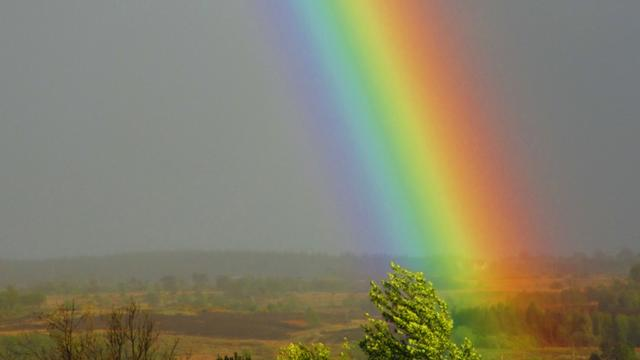
\includegraphics[width=\linewidth]{images/arc_en_ciel.jpg}
\end{center}

En séparant les couleurs qui la composent, les gouttes de pluie dispersent la lumière blanche émise par le Soleil et font apparaitre de magnifiques arcs-en-ciel : on observe ainsi naturellement le \textbf{spectre} de la lumière blanche.
On peut faire de même avec un \textbf{prisme} ou un \textbf{réseau}.
Le spectre du rayonnement émis par un objet permet ensuite d'obtenir des informations sur sa composition, sa température, etc.
\end{multicols}

\section*{Différents types de spectres}

\begin{multicols}{2}
Un spectroscope utilise un réseau pour obtenir le spectre de la lumière issue d'une source.

\noindent
\textcolor{red}{\textbf{\warning{} Ne jamais regarder directement une source intense de lumière comme un laser !}}

\begin{enumerate}
\item \app{} \anarai{}

À l'aide d'un spectroscope, proposer une classification des différentes sources de lumière qui vous entourent (deux catégories).
\end{enumerate}

\begin{center}
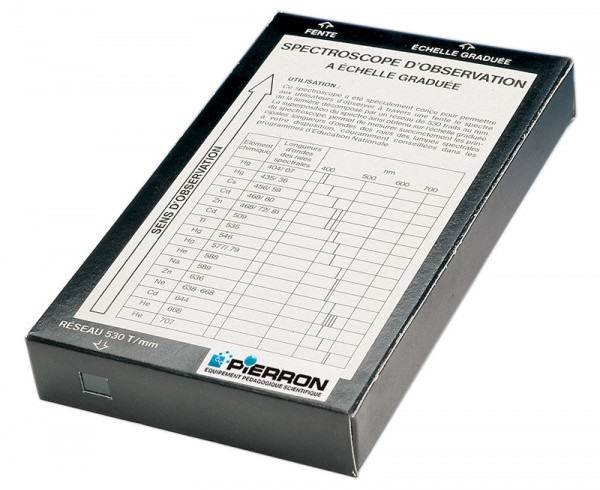
\includegraphics[width=.5\linewidth]{images/spectroscope.jpg}
\end{center}
\end{multicols}

\begin{multicols}{2}
\begin{doc}
\textbf{Spectre continu}

Un corps chaud (la lave, le filament d'une lampe, etc.) émet de la lumière dont le spectre est \textbf{continu}.
Par exemple, le spectre de la lumière émise par le Soleil est semblable à celui-ci :

\begin{center}

\includegraphics[width=\linewidth]{images/sun_spectrum_simple.png}
\end{center}
\end{doc}

\begin{doc}
\textbf{Spectre de raies}

Un gaz excité émet de la lumière dont le spectre n'est pas continu.
On parle de \textbf{spectre de raies d'émissions}.
Par exemple, le spectre d'émission de l'hélium est semblable à celui-ci :

\begin{center}

\includegraphics[width=\linewidth]{images/he_spectrum_simple.png}
\end{center}
\end{doc}
\end{multicols}

\section*{Un nombre pour caractériser la \og couleur \fg{} d'une radiation}

\begin{center}
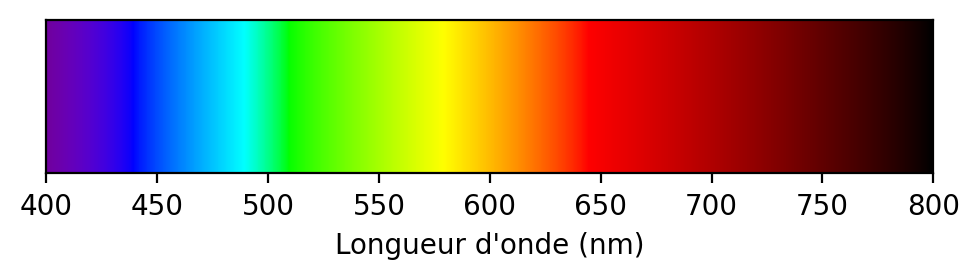
\includegraphics[scale=1]{images/vis_spectrum.png}
\end{center}

\begin{enumerate}
\setcounter{enumi}{1}
\item \app{} \anarai{}

La lampe à vapeur de sodium émet un rayonnement quasi \textbf{monochromatique} (une seule couleur).
Proposer en la justifiant une estimation de la longueur d'onde de ce rayonnement.

\item \rea{} \val{}

Vérifier cette hypothèse avec le spectroscope.
\end{enumerate}

\section*{Que contient la lampe ?}

\begin{enumerate}[resume]
\item \app{} \anarai{} \rea{} \val{} \com{}

Répondre à la question ci-dessus en s'appuyant sur les étapes de la démarche scientifique. 
\end{enumerate}

\begin{appel}
Présenter le protocole avant de réaliser l'expérience.
\end{appel}

\begin{doc}
\textbf{Radiations caractéristiques de quelques espèces}

Le spectre d'émission d'un élément lui est caractéristique.
Le tableau ci-dessous indique la longueur d'onde (en nm) des radiations caractéristiques de quelques espèces.
\begin{center}
\begin{tabular}{|l|c|}
\hline
\textbf{Mercure (Hg)} & 405, 436, 546, 578 \\
\hline
\textbf{Cadmium (Ca)} & 480, 644 \\
\hline
\textbf{Zinc (Zn)} & 468, 472, 481, 636 \\
\hline
\textbf{Hydrogène (H)} & 410, 434, 486, 656 \\
\hline
\end{tabular}
\end{center}
\end{doc}

\section*{Aide à la rédaction du compte-rendu}

\begin{enumerate}
\item \textbf{Hypothèse}. Donnez votre hypothèse et justifiez-la : \og Je pense que ... car ... \fg{}. \hfill \anarai{}

\item \textbf{Protocole}. \hfill \app{} \anarai{} \rea{}

Mettre en place un protocole pour vérifier votre hypothèse. Il peut contenir :
\vspace{-0.5\baselineskip}
\begin{multicols}{2}
\begin{itemize}
\item[•] une expérience :
\begin{enumerate}
\item liste du matériel ;
\item schémas ;
\item observations et mesures ;
\end{enumerate}
\item[•] un calcul :
\begin{enumerate}
\item formule littérale ;
\item conversion ;
\item application numérique ;
\end{enumerate}
\end{itemize}
\end{multicols}
\vspace{-1.\baselineskip}
\begin{itemize}
\item[•] un raisonnement, une étude de documents, etc.
\end{itemize}
\item \textbf{Conclusion}. Pour terminer le compte-rendu : \hfill \val{}
\begin{itemize}
\item[•] donner les conclusions en reprenant ce qui a été trouvé dans le protocole ;
\item[•] dire si les conclusions sont en accord avec votre hypothèse ;
\item[•] répondre à la question posée !
\end{itemize}
\end{enumerate}

\end{document}

\begin{doc}
\textbf{Spectres d'émission de quelques espèces}

Le spectre d'émission d'un élément lui est caractéristique : voici ceux de quelques espèces.
\begin{center}
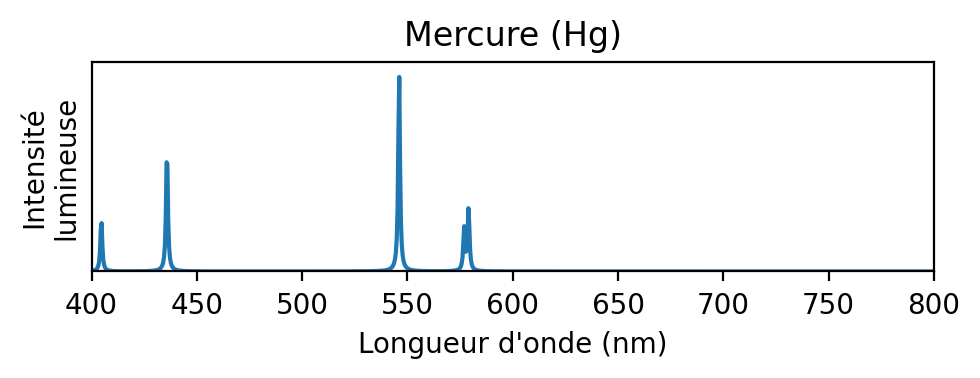
\includegraphics[width=.49\linewidth]{images/spectrum_curve_Hg.png}
\hfill
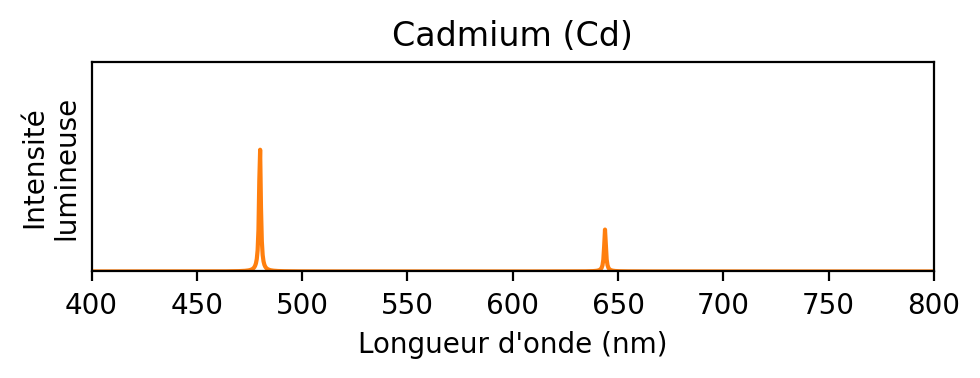
\includegraphics[width=.49\linewidth]{images/spectrum_curve_Cd.png}

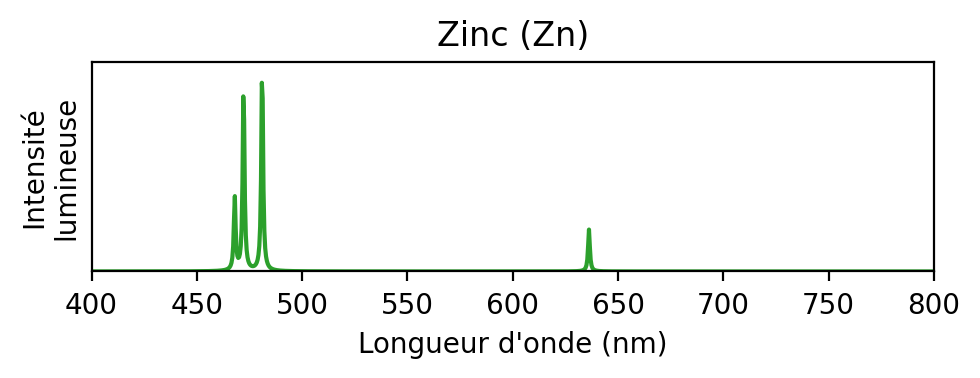
\includegraphics[width=.49\linewidth]{images/spectrum_curve_Zn.png}
\hfill
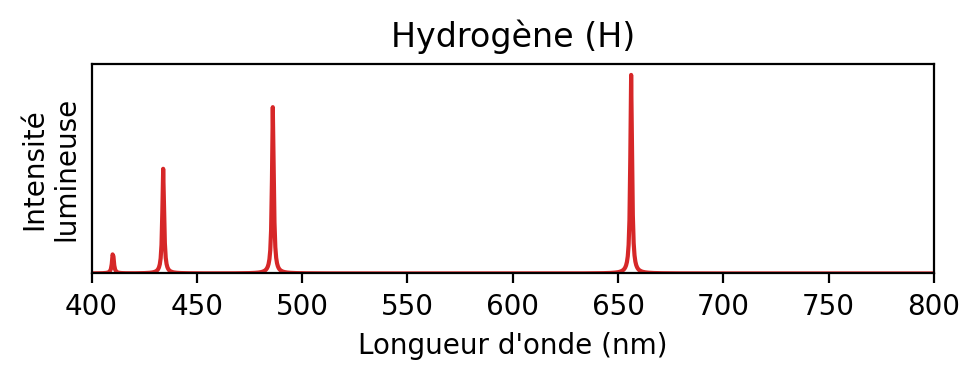
\includegraphics[width=.49\linewidth]{images/spectrum_curve_H.png}
\end{center}
\end{doc}

\begin{doc}
\textbf{Spectre d'émission de quelques espèces}

Le spectre d'émission d'un élément lui est caractéristique : voici ceux de quelques espèces.
\begin{center}
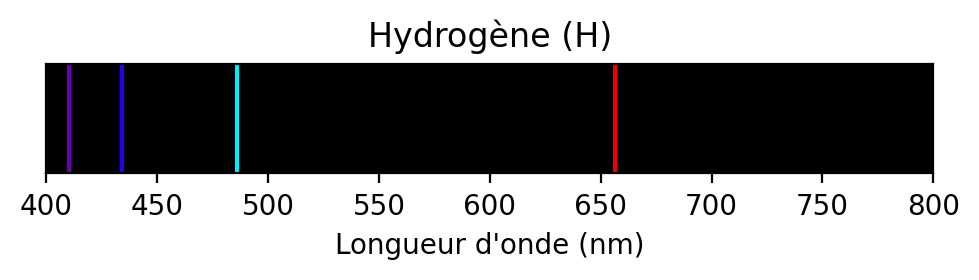
\includegraphics[width=.49\linewidth]{images/spectrum_H.png}
\hfill
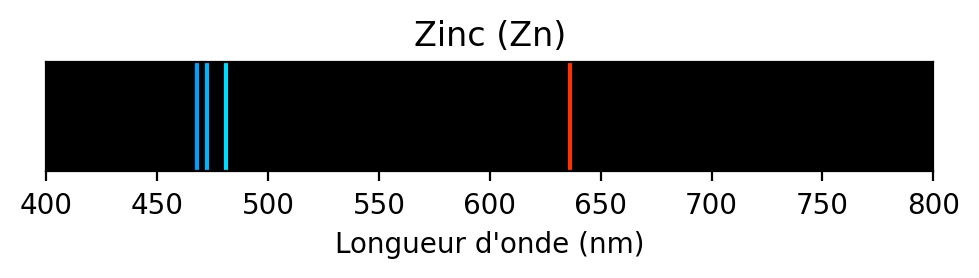
\includegraphics[width=.49\linewidth]{images/spectrum_Zn.png}

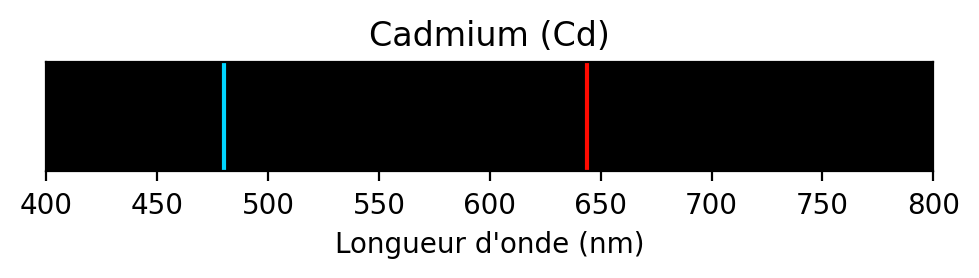
\includegraphics[width=.49\linewidth]{images/spectrum_Cd.png}
\hfill
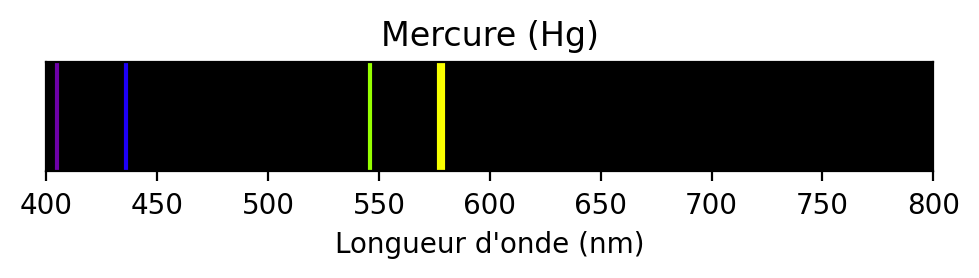
\includegraphics[width=.49\linewidth]{images/spectrum_Hg.png}
\end{center}
\end{doc}

% Demander si certains ont des problème avec les couleurs

% Contextualisation

% Pendant 15 min, observer le spectre des lumières provenant des sources qui vous entourent. Comment pourrait-on les classer ?